%%%%%%%%%%%%%%%%%%%%%%%%%%%%%%%%%%%%%%%%%
% Thin Sectioned Essay
% LaTeX Template
% Version 1.0 (3/8/13)
%
% This template has been downloaded from:
% http://www.LaTeXTemplates.com
%
% Original Author:
% Nicolas Diaz (nsdiaz@uc.cl) with extensive modifications by:
% Vel (vel@latextemplates.com)
%
% License:
% CC BY-NC-SA 3.0 (http://creativecommons.org/licenses/by-nc-sa/3.0/)
%
%%%%%%%%%%%%%%%%%%%%%%%%%%%%%%%%%%%%%%%%%

%----------------------------------------------------------------------------------------
%	PACKAGES AND OTHER DOCUMENT CONFIGURATIONS
%----------------------------------------------------------------------------------------

\documentclass[a4paper, 11pt]{article} % Font size (can be 10pt, 11pt or 12pt) and paper size (remove a4paper for US letter paper)
\usepackage{float}
\usepackage[protrusion=true,expansion=true]{microtype} % Better typography
\usepackage{graphicx} % Required for including pictures
\usepackage{wrapfig} % Allows in-line images
\usepackage{indentfirst}
\usepackage{mathpazo} % Use the Palatino font
\usepackage[T1]{fontenc} % Required for accented characters
\usepackage{subfigure}
\usepackage{amsmath}
\usepackage{amssymb}
\usepackage{mathtools}
\usepackage{listings}
\usepackage{xcolor}
\usepackage[framemethod=default]{mdframed}
\usepackage[noend]{algpseudocode}
\usepackage{algorithmicx,algorithm}
\usepackage{times} 
\usepackage{CJK} 
\usepackage{wrapfig}
\usepackage{amsmath,amssymb} 

\newtheorem{definition}{{Definition}}

\linespread{1.05} % Change line spacing here, Palatino benefits from a slight increase by default

\makeatletter
\renewcommand\@biblabel[1]{\textbf{#1.}} % Change the square brackets for each bibliography item from '[1]' to '1.'
\renewcommand{\@listI}{\itemsep=0pt} % Reduce the space between items in the itemize and enumerate environments and the bibliography

\renewcommand{\maketitle}{ % Customize the title - do not edit title and author name here, see the TITLE block below
\begin{flushright} % Right align
{\LARGE\@title} % Increase the font size of the title

\vspace{50pt} % Some vertical space between the title and author name

{\large\@author} % Author name
\\\@date % Date

\vspace{40pt} % Some vertical space between the author block and abstract
\end{flushright}
}

\title{\textbf{A Convolutional Model for Tone Classification}\\ \vspace{0.5cm}
{Final Project of MS318, Fall 2016}} 

\author{\textsc{Xueyuan Zhao, Haoming Lu, Yunqi Li} 
\\{\textit{}}} 

\date{\today} 

\begin{document}

\maketitle

\begin{abstract}
To improve the tone classification on Mandarin Chinese individual characters, we proposed a model with data processing and convolutional model which focuses on reducing the noise in the dataset. Given a specific character, this approach excludes noise frames by both frequency and energy information, regenerates the frequency sequence by spline fitting, captures the feature and finally acts the classification with a convolutional neural network (CNN).  We evaluated our model on the provided datasets \textit{test} and \textit{test\_new}, achieved the accuracy of $\mathbf{100\%}$ and $\mathbf{98.25\%}$ respectively within a short period of time.
\end{abstract}

\vspace{30pt} 

\section{Introduction}
\indent
Chinese language is a tonal language while the tonal system of Mandarin Chinese has four lexical tone patterns including (1) flat and high, (2) rising, (3) low and dipping, and (4) falling, which can be reflected through the fundamental frequency(F0) variation over time. 
\par
Some previous works on this problem tend to extract feature vector of the data and then deal with it by support vector machine (SVM)\cite{wang2009tone} or some even more direct apporaches. However, considering the course mostly focuses on deep learning, we decided to keep the preprocessed input sequence and construct a neural network to finish the rest of the work, which turned out to be an effective idea. We will introduce how we preprocess the input data in \textbf{Chapter 2}, the network model in \textbf{Chapter 3}. The experiment results and comparation among different toolkits will be presented in \textbf{Chapter 4}. And \textbf{Chapter 5} will be a summary to our work.

\section{Data Processing}
After reading the dataset and referring some previous works, we noticed that most mistakes in this problem are caused by environmental noise and pronunciation differences among people. In order to deal with these disturbance, we executed \textit{invalid frame exclusion}, \textit{difference normalization} and \textit{spline fitting} successively. The network designed for this way of processing turned out to perform best among all the ways we had tried. We will then discuss the three parts in detail.
\\
\subsection{Invalid Frame Exclusion}
Both the environmental noise and pronunciation patterns lead to invalid frames. From the frequency input of training dataset, we can see that each sequence has a series of zero frames in the front and in the tail. It is not hard to see that these frames are useless in distinguishing tones, so we set a constant $threshold_{f0}$, all the frames where the value is less than $threshold_{f0}$ will be ignored. And from energy input of training dataset we discovered that, the values of some frames are extremely small which indicates that the corresponding frames in the frequency sequence also make no sense. These frames are also excluded according to another constant $threshold_{en}$. In the end, considering that the pronouncing process may not be stable in the beginning or in the end, we exclude a few frames at both ends.
\par
The whole process can be implemented with the following Python code:
\vspace{0.5cm}
\begin{mdframed}[skipabove=7pt,
	skipbelow=7pt,
	rightline=false,
	leftline=true,
	topline=false,
	bottomline=false,
	linecolor=gray,
	backgroundcolor=black!5,
	innerleftmargin=5pt,
	innerrightmargin=5pt,
	innertopmargin=-3pt,
	innerbottommargin=-5pt,
	leftmargin=0cm,
	rightmargin=0cm,
	linewidth=4pt]
\begin{lstlisting}[language=Python]
def exclude_invalid_frame(f0, en):
  f0 = f0[numpy.where(en < en_threshold)[0]]
  f0 = f0[numpy.where(f0 < f0_threshold)[0]]
  f0 = f0[cut_length:-cut_length]
  return f0
\end{lstlisting}
\end{mdframed}
\begin{figure}[H]
\begin{minipage}{0.5\linewidth}
\centerline{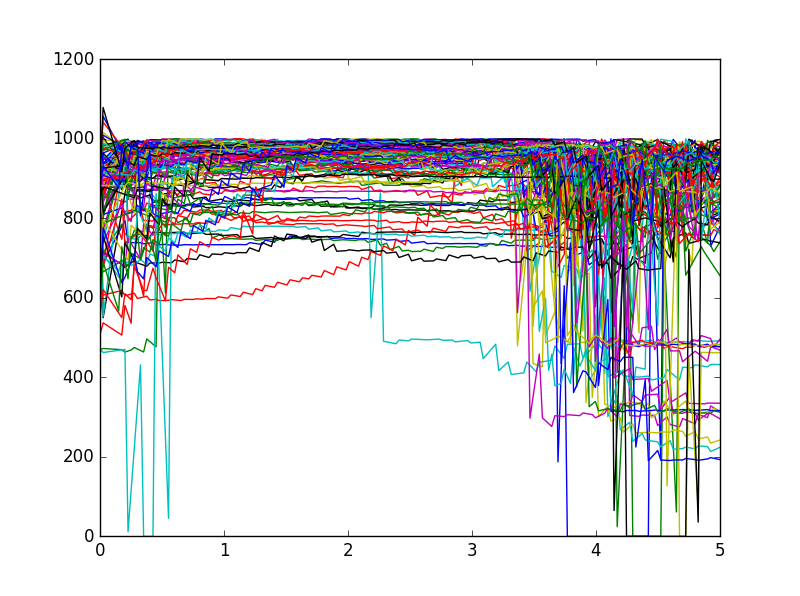
\includegraphics[width=6.0cm]{figure/originf0_1.png}}
\end{minipage}
\hfill
\begin{minipage}{0.5\linewidth}
\centerline{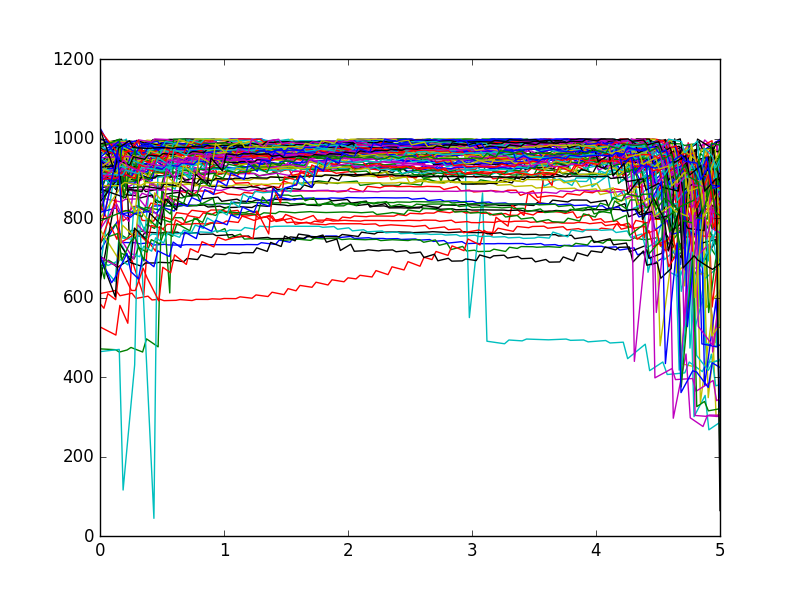
\includegraphics[width=6.0cm]{figure/exclude_1.png}}
\end{minipage}
\vfill
\begin{minipage}{0.5\linewidth}
\centerline{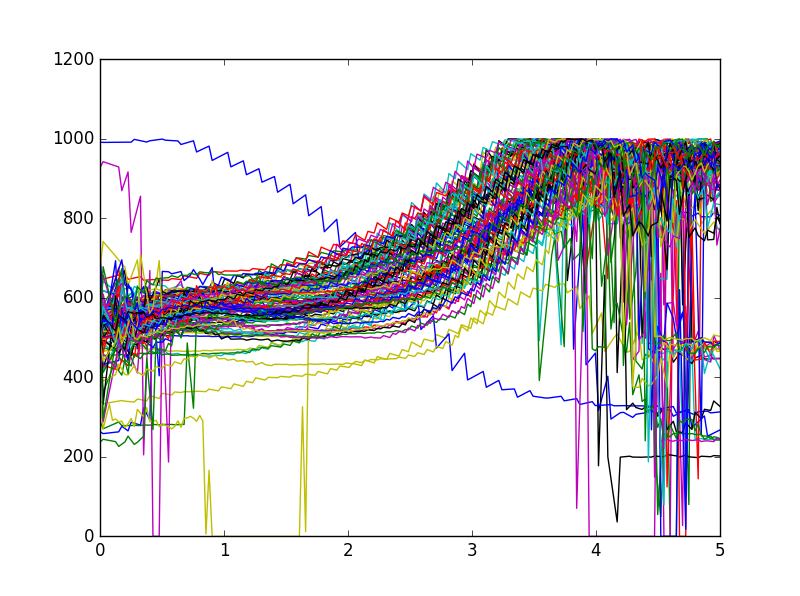
\includegraphics[width=6.0cm]{figure/originf0_2.png}}
\end{minipage}
\hfill
\begin{minipage}{0.5\linewidth}
\centerline{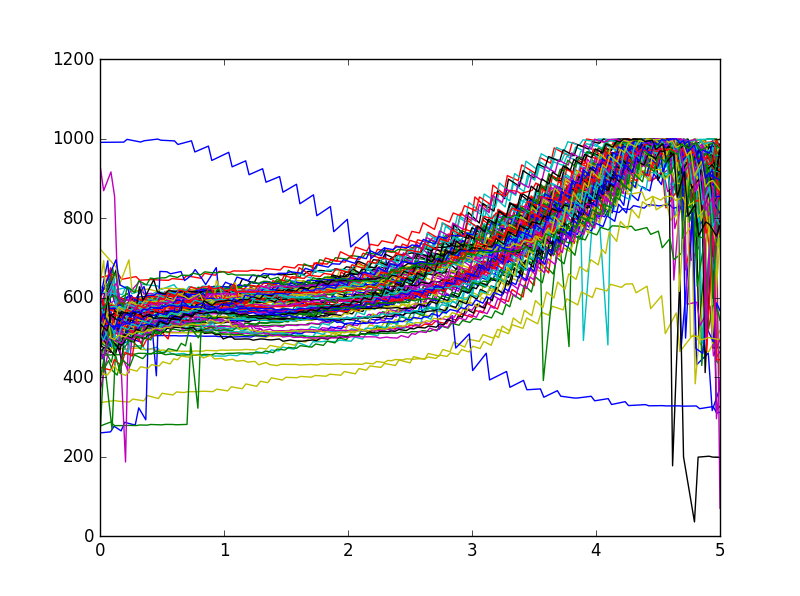
\includegraphics[width=6.0cm]{figure/exclude_2.png}}
\end{minipage}
\begin{minipage}{0.5\linewidth}
\centerline{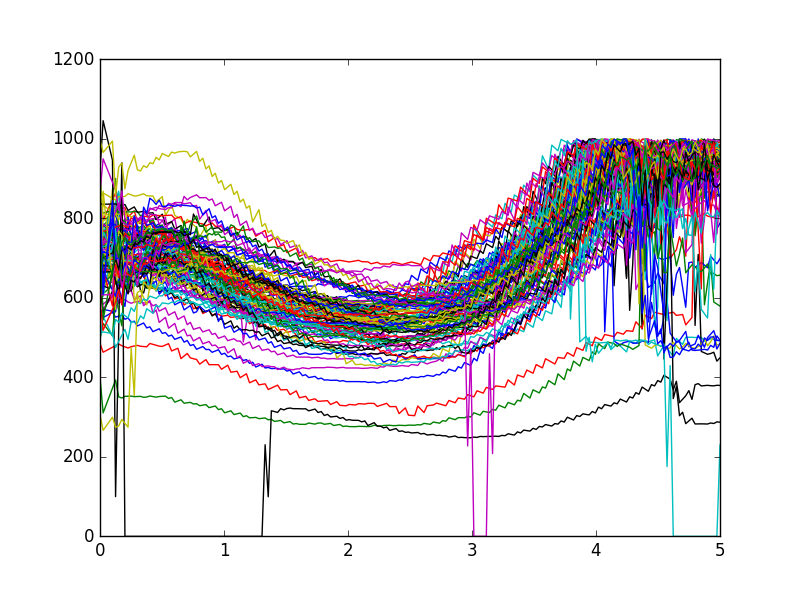
\includegraphics[width=6.0cm]{figure/originf0_3.png}}
\end{minipage}
\hfill
\begin{minipage}{0.5\linewidth}
\centerline{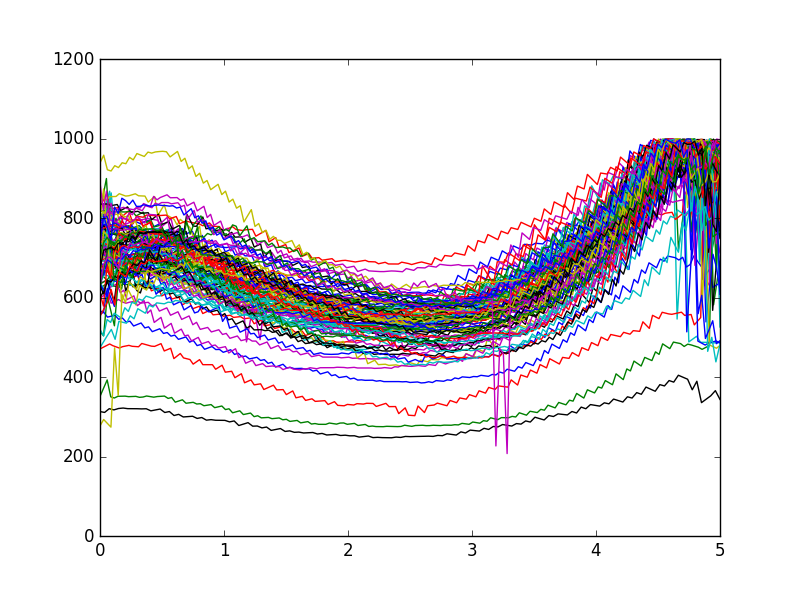
\includegraphics[width=6.0cm]{figure/exclude_3.png}}
\end{minipage}
\vfill
\begin{minipage}{0.5\linewidth}
\centerline{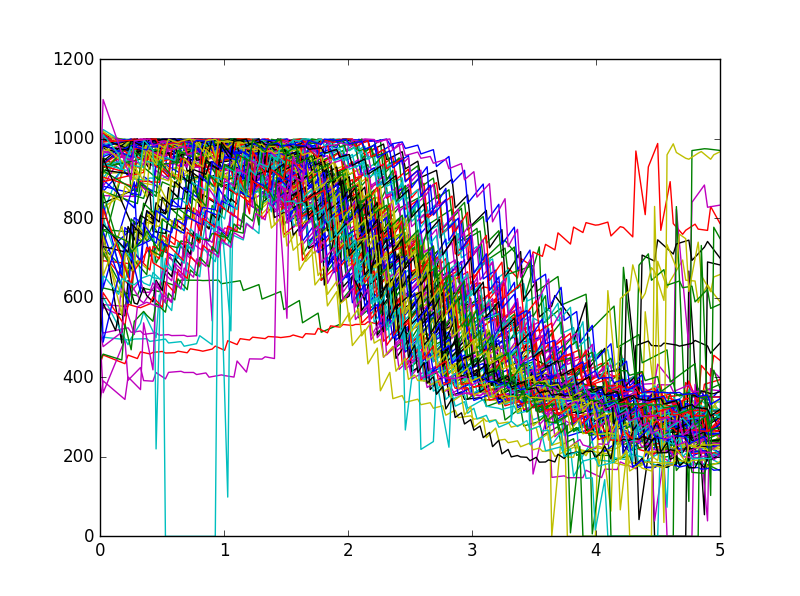
\includegraphics[width=6.0cm]{figure/originf0_4.png}}
\end{minipage}
\hfill
\begin{minipage}{0.5\linewidth}
\centerline{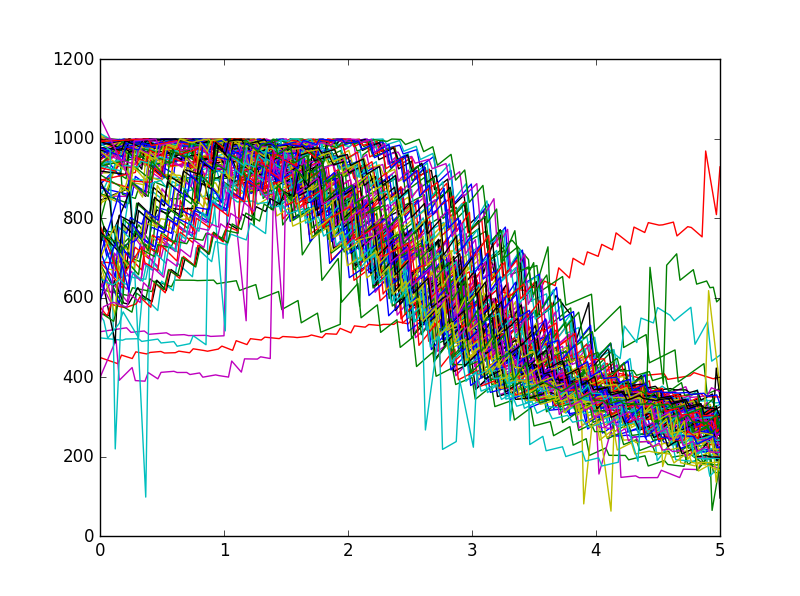
\includegraphics[width=6.0cm]{figure/exclude_4.png}}
\end{minipage}
\caption{The comparation between original frequency sequences(left) and excluded sequences(right). The data are captured from training dataset.}
\label{fig_originf0}
\end{figure}
\newpage
\subsection{Difference Normalization}
After observing the input fundamental frequencies of the training dataset (as shown in Figure 1), we found that, most lines with the same label already share similar patterns except some variance in the $y$ direction. So we decided to do the first order difference along the x-axis as
$$ f0_{dif}(i) = f0(i+1) - f0(i) $$
\par
We then noticed that most of the difference sequences with the same label have similar tendencies over time. However, the distribution of actual numerical values of first order differences has high variance which might have a negative influence on the performance of network models.  In order to reduce the variance of first order difference sequences, we set a threshold $bound$ and replaced all the frames where the absolute value is beyond the threshold with it. This method can be described as
\begin{equation}
    f0_{norm\_ dif}(i)=
   \begin{cases}
bound, & f0_{dif}(i) > bound \cr
-bound, & f0_{dif}(i) < -bound \cr
f0_{dif}(i), & otherwise
   \end{cases}
\end{equation}
\par
Figure 2 shows the comparison between original difference and the differences after normalization.
\vspace{1cm}
\subsection{Spline Fitting}
The replacement above indeed excluded abnormal frames, but it broke the continuity of the sequence in some ways. In order to reconstruct the continuity and eventually smooth the frequency sequences, we applied interpolations here to regenerate the sequence. After attempting different kinds of interpolations including polynomial interpolation, Hermite interpolation and spline interpolation, cubic spline interpolation, as defined below, turned out to have the best performance among them in testing.
\begin{definition}
The cubic spline interpolation of n points $(x_i,y_i)$ is defined as n cubic polynomials $p_i(x)$, where\\
$$p_i(x_i)=y_i$$
$$p_i(x_{i+1})=y_{i+1}$$
$$p'_i(x_{i+1})=p'_{i+1}(x_{i+1})$$
$$p''_i(x_{i+1})=p''_{i+1}(x_{i+1})$$
\end{definition}
\par
More narrowly, we first set all the values uniformly on a interval with fixed length, for example $[0,100]$, and used their new coordinates as the input data. After excuting interpolation, we then resampled on a fixed numer of positions in this intervel, for example, all the integer points, now all the frequency sequences will have the same length.
\par
The Figure 3 following gives comparation between the original frequency sequences and frequency sequences recovered from the preprocessed differences. The left column came from the original data while the right column are recovered from the preprocessed difference, with the start value fixed to zero. We can see that features of different labels became much more distinct after data processing.
\begin{figure}[H]
\begin{minipage}{0.5\linewidth}
\centerline{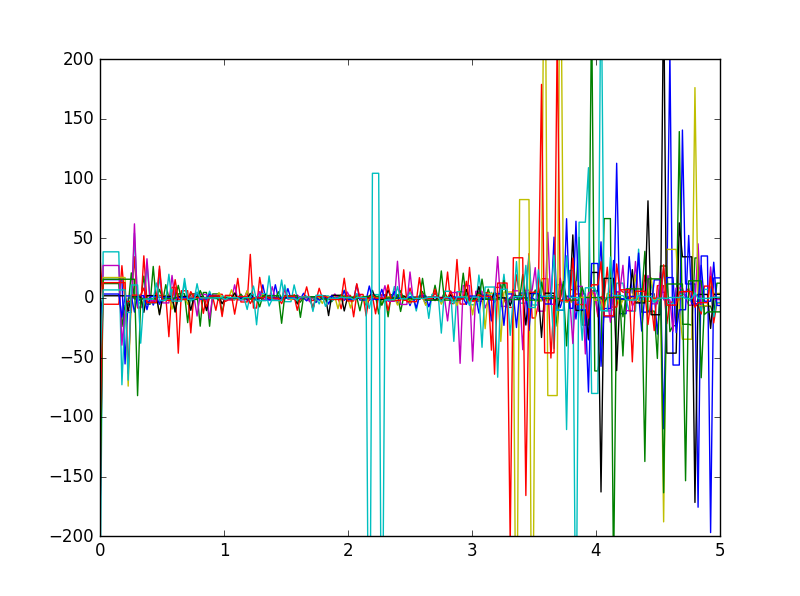
\includegraphics[width=6.0cm]{figure/dif_1.png}}
\end{minipage}
\hfill
\begin{minipage}{0.5\linewidth}
\centerline{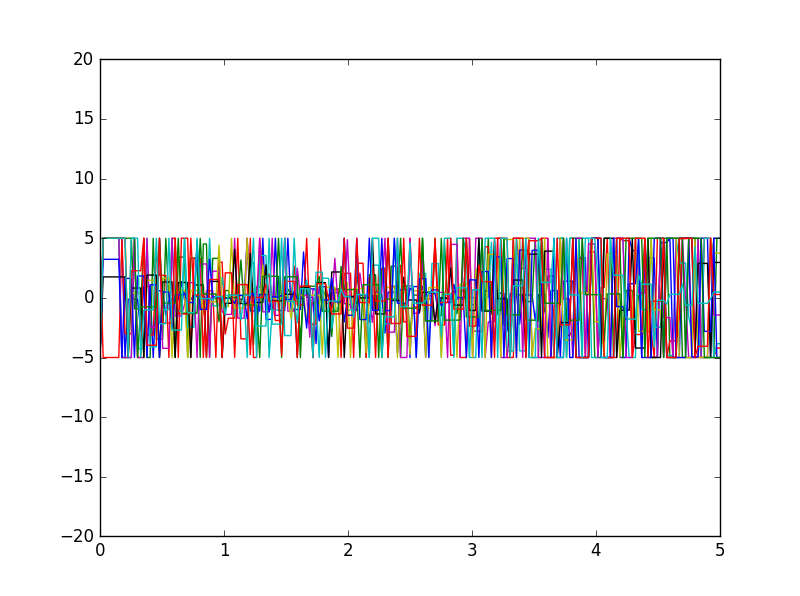
\includegraphics[width=6.0cm]{figure/fitdif_1.png}}
\end{minipage}
\vfill
\begin{minipage}{0.5\linewidth}
\centerline{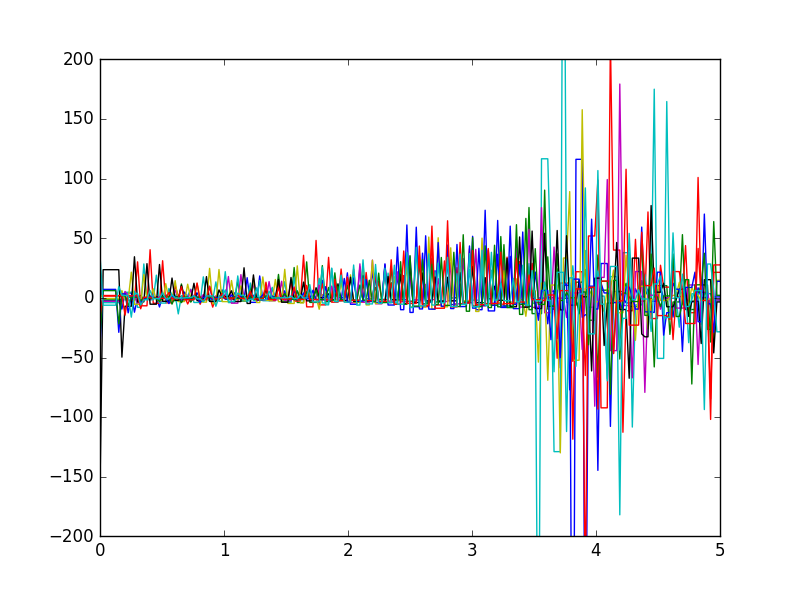
\includegraphics[width=6.0cm]{figure/dif_2.png}}
\end{minipage}
\hfill
\begin{minipage}{0.5\linewidth}
\centerline{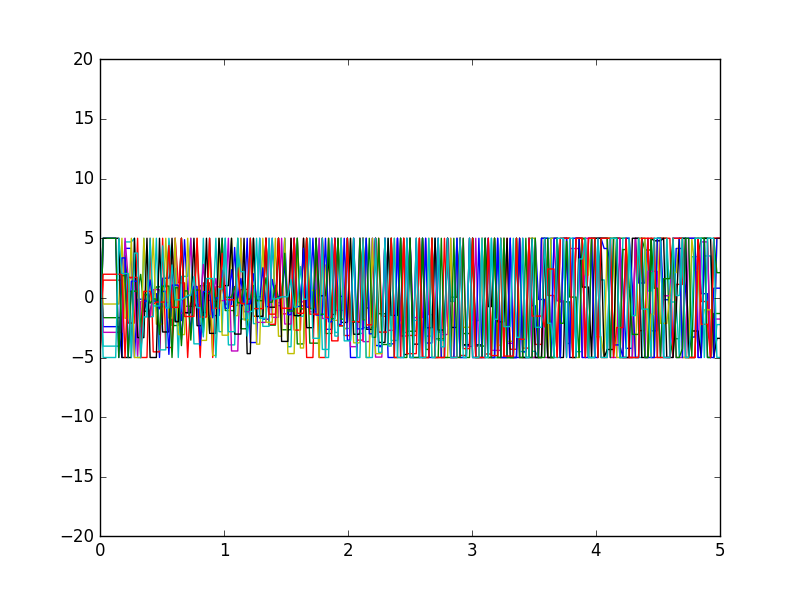
\includegraphics[width=6.0cm]{figure/fitdif_2.png}}
\end{minipage}
\begin{minipage}{0.5\linewidth}
\centerline{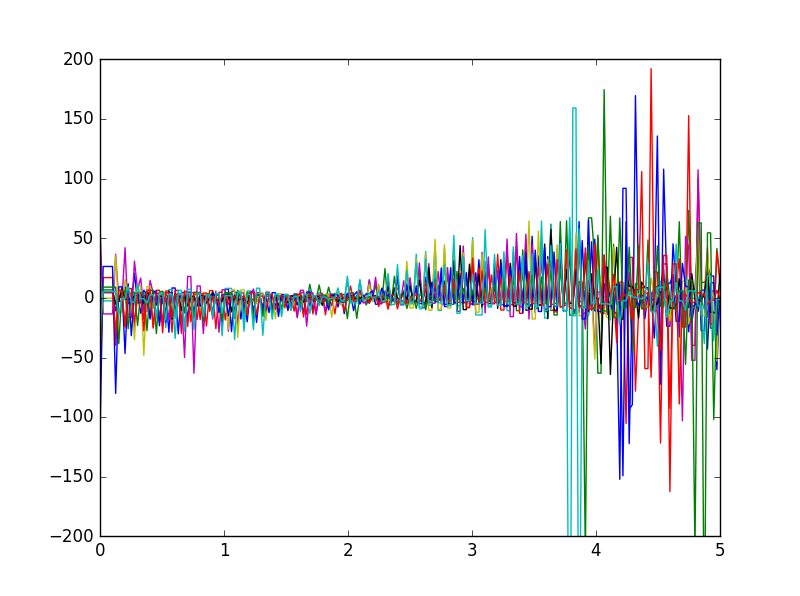
\includegraphics[width=6.0cm]{figure/dif_3.png}}
\end{minipage}
\hfill
\begin{minipage}{0.5\linewidth}
\centerline{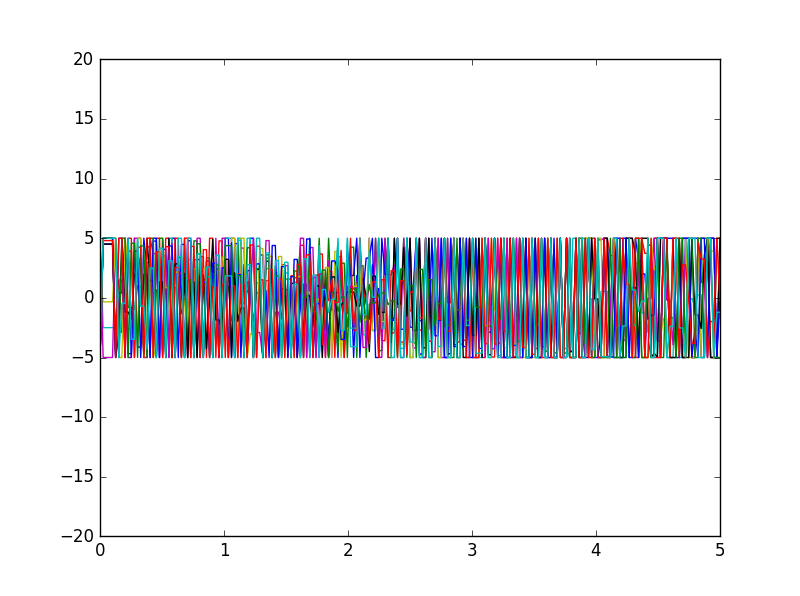
\includegraphics[width=6.0cm]{figure/fitdif_3.png}}
\end{minipage}
\vfill
\begin{minipage}{0.5\linewidth}
\centerline{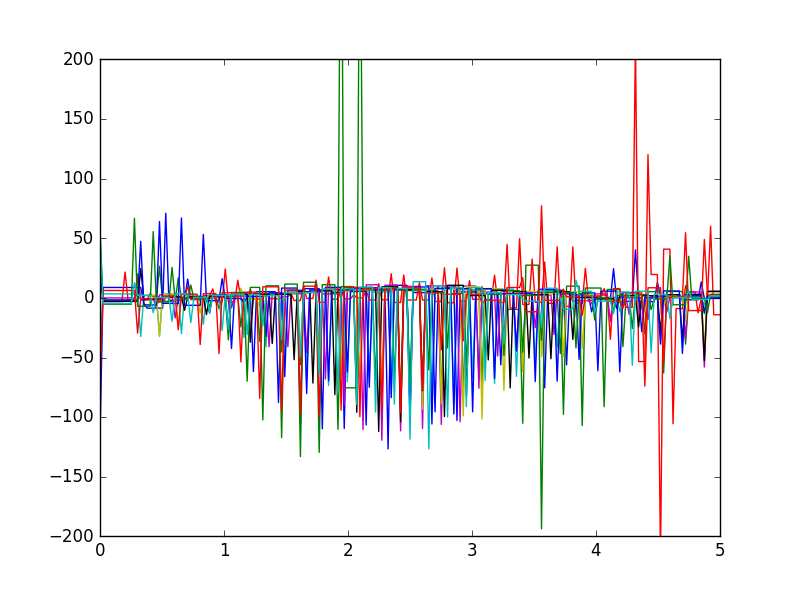
\includegraphics[width=6.0cm]{figure/dif_4.png}}
\end{minipage}
\hfill
\begin{minipage}{0.5\linewidth}
\centerline{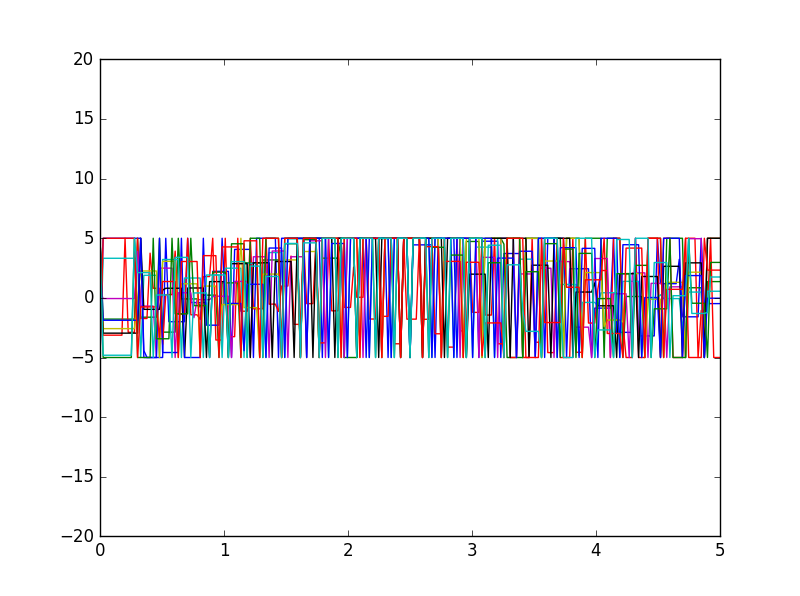
\includegraphics[width=6.0cm]{figure/fitdif_4.png}}
\end{minipage}
\caption{Comparation between original differences and normalized differences. 10 examples per label are picked. Notice that the axis ranges on the left side are ten times those on the right side.}
\label{fig_f0fit}
\end{figure}

\begin{figure}[H]
\begin{minipage}{0.5\linewidth}
\centerline{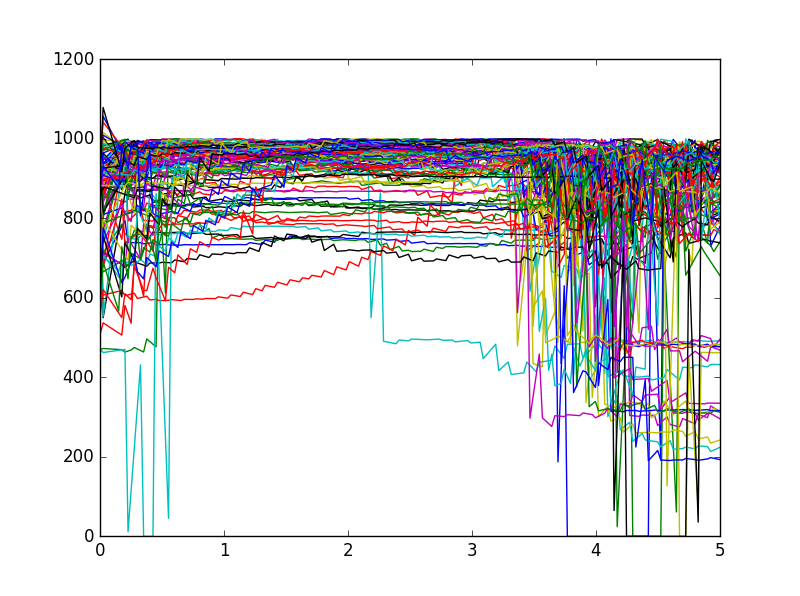
\includegraphics[width=6.0cm]{figure/originf0_1.png}}
\end{minipage}
\hfill
\begin{minipage}{0.5\linewidth}
\centerline{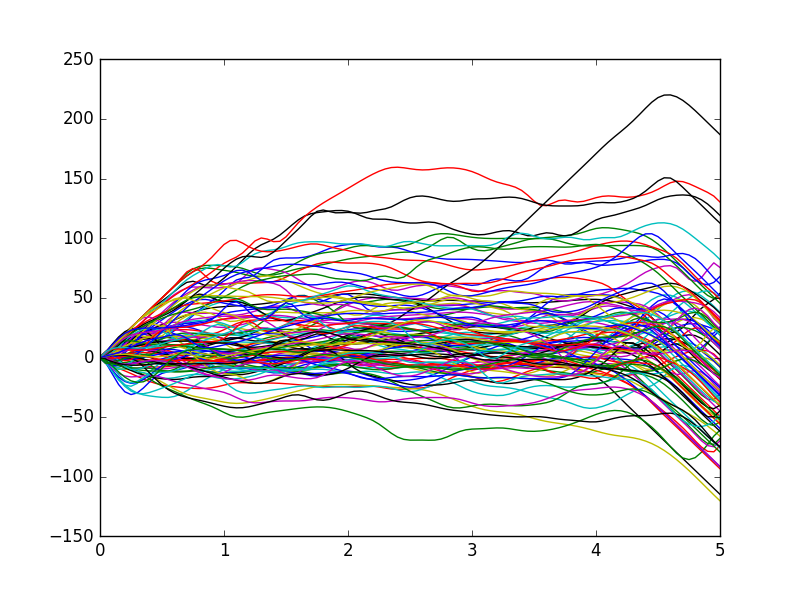
\includegraphics[width=6.0cm]{figure/finalnorm_1.png}}
\end{minipage}
\vfill
\begin{minipage}{0.5\linewidth}
\centerline{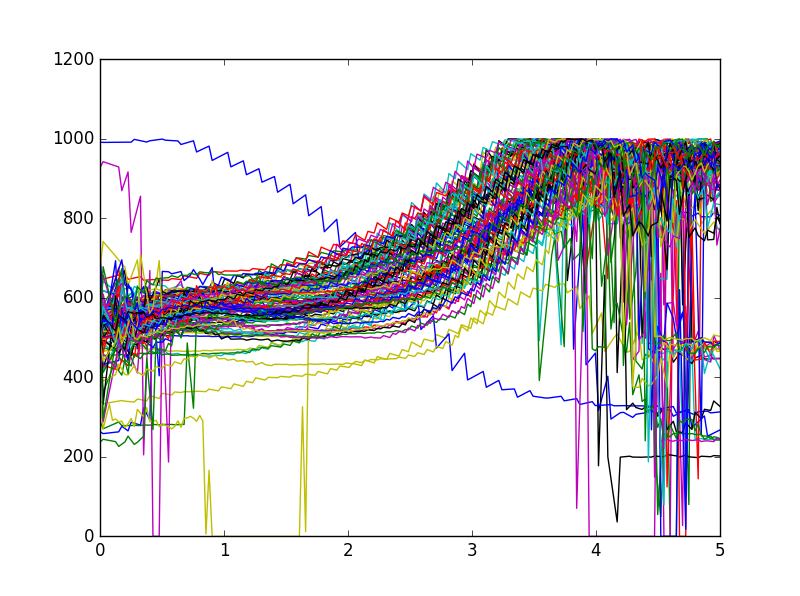
\includegraphics[width=6.0cm]{figure/originf0_2.png}}
\end{minipage}
\hfill
\begin{minipage}{0.5\linewidth}
\centerline{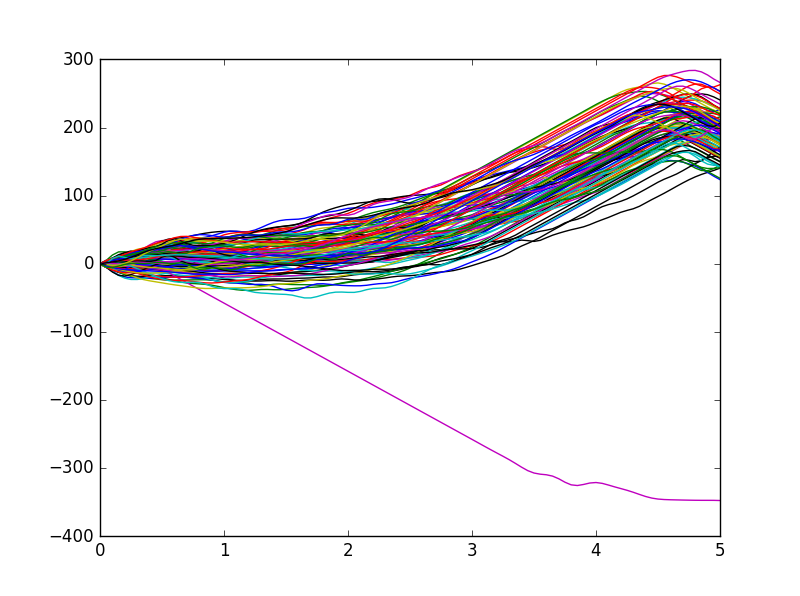
\includegraphics[width=6.0cm]{figure/finalnorm_2.png}}
\end{minipage}
\vfill\begin{minipage}{0.5\linewidth}
\centerline{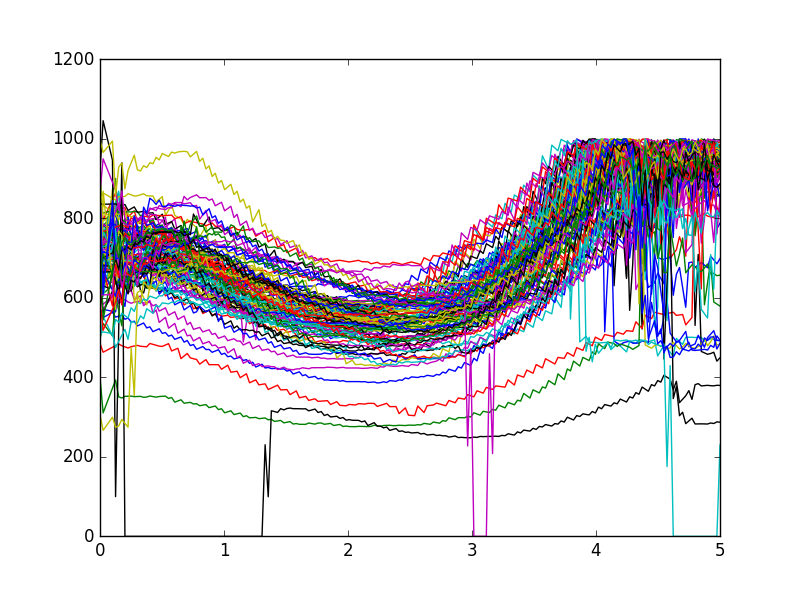
\includegraphics[width=6.0cm]{figure/originf0_3.png}}
\end{minipage}
\hfill
\begin{minipage}{0.5\linewidth}
\centerline{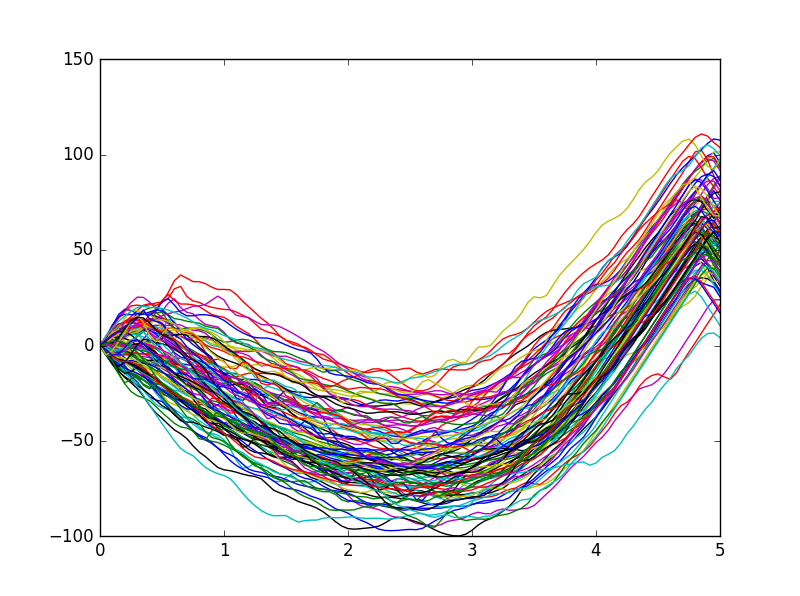
\includegraphics[width=6.0cm]{figure/finalnorm_3.png}}
\end{minipage}
\vfill\begin{minipage}{0.5\linewidth}
\centerline{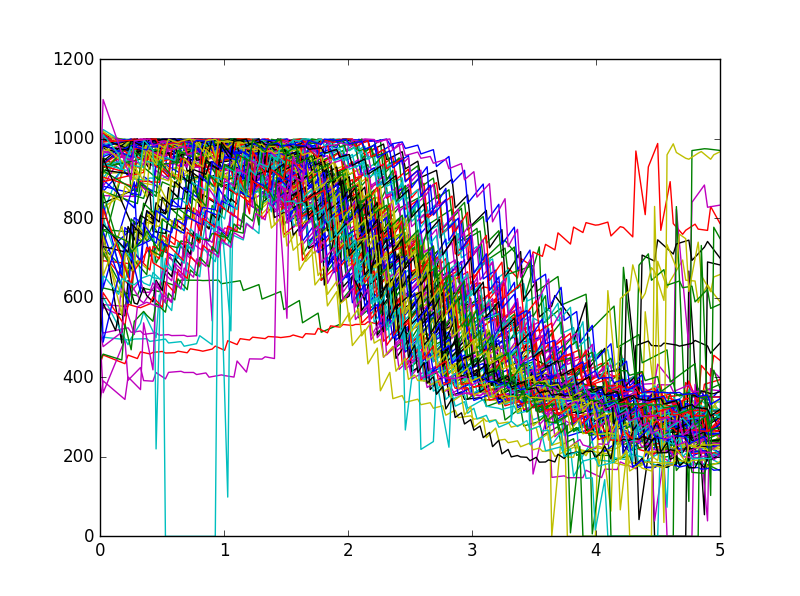
\includegraphics[width=6.0cm]{figure/originf0_4.png}}
\end{minipage}
\hfill
\begin{minipage}{0.5\linewidth}
\centerline{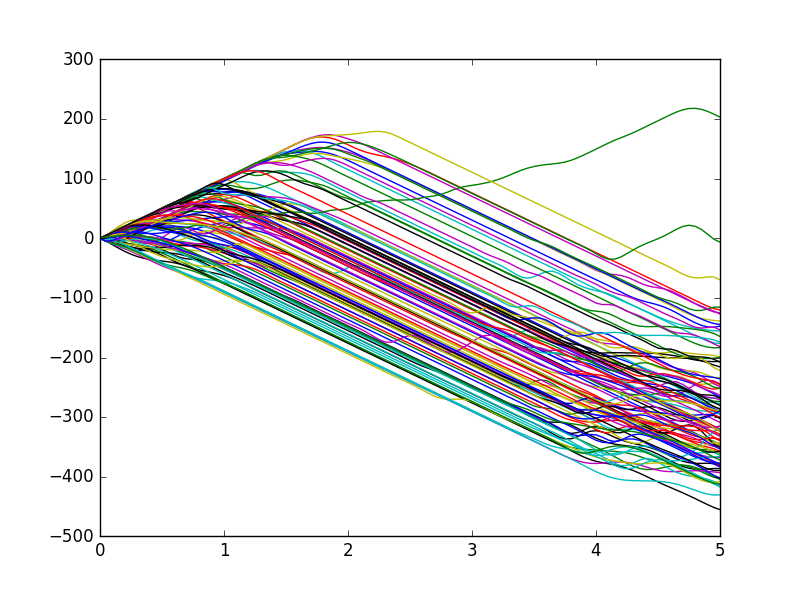
\includegraphics[width=6.0cm]{figure/finalnorm_4.png}}
\end{minipage}
\vfill
\caption{Comparation between the original and preprocessed frequency sequences on training dataset. Notice that the subfigures in the right column are suitably scaled to make the tendency more evident.}
\label{fig_f0compare}
\end{figure}

\section{Network Model}
We implemented several neural network models on this problem. Our first attempt with deep neural network (DNN) including two fully-connected hidden layers achieved 100\% accuracy on dataset \textit{test}, but it turned out to perform poor on dataset \textit{test\_new}. After further experiments with recurrent neural networks (RNN)\cite{goller1996learning} and convolutional neural networks (CNN), we found that CNN performed better no matter from the consideration on time or on accuracy, and eventually proposed a convolutional net model with 8 hidden layers. Figure 4 desribes the architecture of the network.
\par
The input of the network is a 1-D vector of length $100$, preprocessed with $threshold_{f0} = 50.0$., $threshold_{en} = 50.0$, $cut\_len = 3$ and $bound = 5.0$. The kernel size of convolutional layers and max-pooling layers are $[10,]$ and $[4,]$ respectively. The performance of the model increases until 3 Conv-Pool blocks are piled up. The convolutional layers are initialized with uniform distribution on $[-0.97, 0.97]$ and padded with zero. Two fully connected layers each with 2048 units and use $sigmoid$ for activation are foillowing.
\par
We trained the model with 10 batchsize Stochastic Gradient Descent (SGD)\cite{lecun1989backpropagation} and learning rate 0.005. The model converges after about 60 epochs. All the parameters were adjusted according to the architecture and input data, some processes of adjustment will be introduced in the next section.
\begin{figure}[H]
\begin{minipage}{1\linewidth}
\centerline{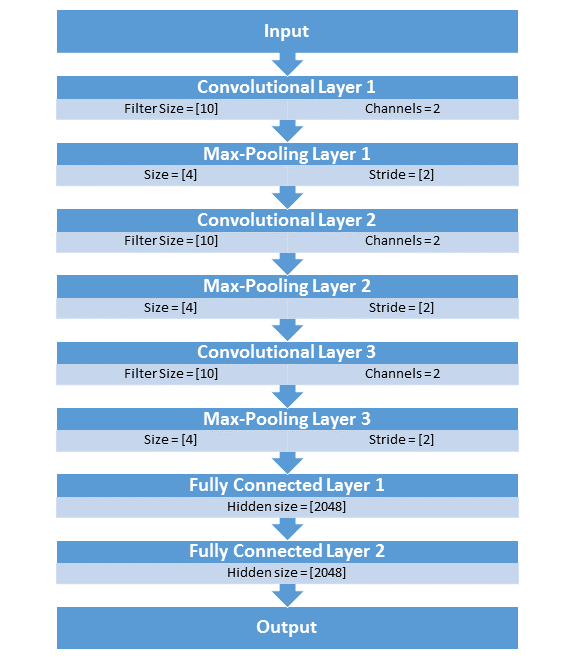
\includegraphics[width=17.0cm]{figure/arch.png}}
\end{minipage}
\caption{The Architecture of Network Model}
\label{arch}
\end{figure}

\section{Experiments}
In this section, we present our experiments in details, including processing, experimental setup, model comparison, toolkit comparison, and corresponding analysis. Since almost all of our models can reach the accuracy of more than $\mathbf{99\%}$ on the easy data set \textit{test}, we will only discuss the performances on the hard data set \textit{test\_new}. In our experiments, our model reached the accuracy of $\mathbf{98.25\%}$ on \textit{test\_new}.
\subsection{Datasets}
The dataset consists of three parts: \textit{train}, \textit{test} and \textit{test\_new}. The \textit{train} and \textit{test} are the voices of standard Mandarin recorded in the quite environment. The \textit{text\_new} are the voices of Mandarin (may have accent) recorded in the normal office environment. 
\subsection{Evaluation Metrics}
The main evaluation metric in our experiment is classification accuracy, which is the ratio of correct classification predictions :
\[
	\text{Accuracy} = \frac{\text{Number of Correct Predictions}}{\text{Total Number of  Predictions}} \times 100\%
\]
\subsection{Comparison over Data Process Methods}
In our experiments, we tested the three data process methods mentioned in \textbf{Chapter 2}. In this section, we call the corresponding three methods \textit{Exclude}, \textit{Normalize} and \textit{Fit}. The relationship between accuracy and data process methods are shown in Figure 5.
\subsection{Comparison over Model Architectures}
In this section, we discuss the impact of model architecture. For our convolutional models, we take three hyperparameters into consideration:
\begin{enumerate}
	\item \textit{Width of Network}: We explore the impact of network width by adjusting the width of fully connected layers in our model. We compared different widths of fully connected layers:  $2^8$, $2^9$, $2^{10}$, $2^{11}$, $2^{12}$ and $2^{13}$. Figure 6 (Left) shows the performance as network width grows. Generally speaking, the networks with fully connected layers of width $2^{11}$ works better generalization on the test set.
	\item \textit{Network Depth}: We explore the impact of network depth by adjusting the depth of fully connected layers in our model. We compared different depths of fully connected layers:  $1$, $2$, $3$ and $4$. Figure 6 (Right) shows the performance as network depth grows. Generally speaking, the networks with fully connected layers of depth $2$ works better generalization on the test set.

	\item \textit{Activation Functions}: In our experiments, we compared three mainstream activation functions: $\text{sigmoid}(x)=\frac{1}{1+e^{-x}}$, $\tanh(x)=\frac{1-e^{-2x}}{1+e^{-2x}}$ and $\text{relu}(x)=\max(0,x)$. Figure 7 (right) compares these activation functions on our model. From this figure we find that sigmoid has better performance than tanh and relu.
	\item \textit{Number of Convolution Filters}: In our model, there are 3 convolutional layers, we explore the impact of different number of convolutional filters by comparing following parameters (x-y-z means the first convolutional layer has x filters, the second convolutional layer has y filters, the third convolutional layer has z filters): 1-2-4, 2-4-8, 4-8-16 and 8-16-32. The results are shown in the Figure 7 (left). The results show that the set of parameters 2-4-8 outperforms other sets.
	
\end{enumerate}

\begin{figure}[H]
\centerline{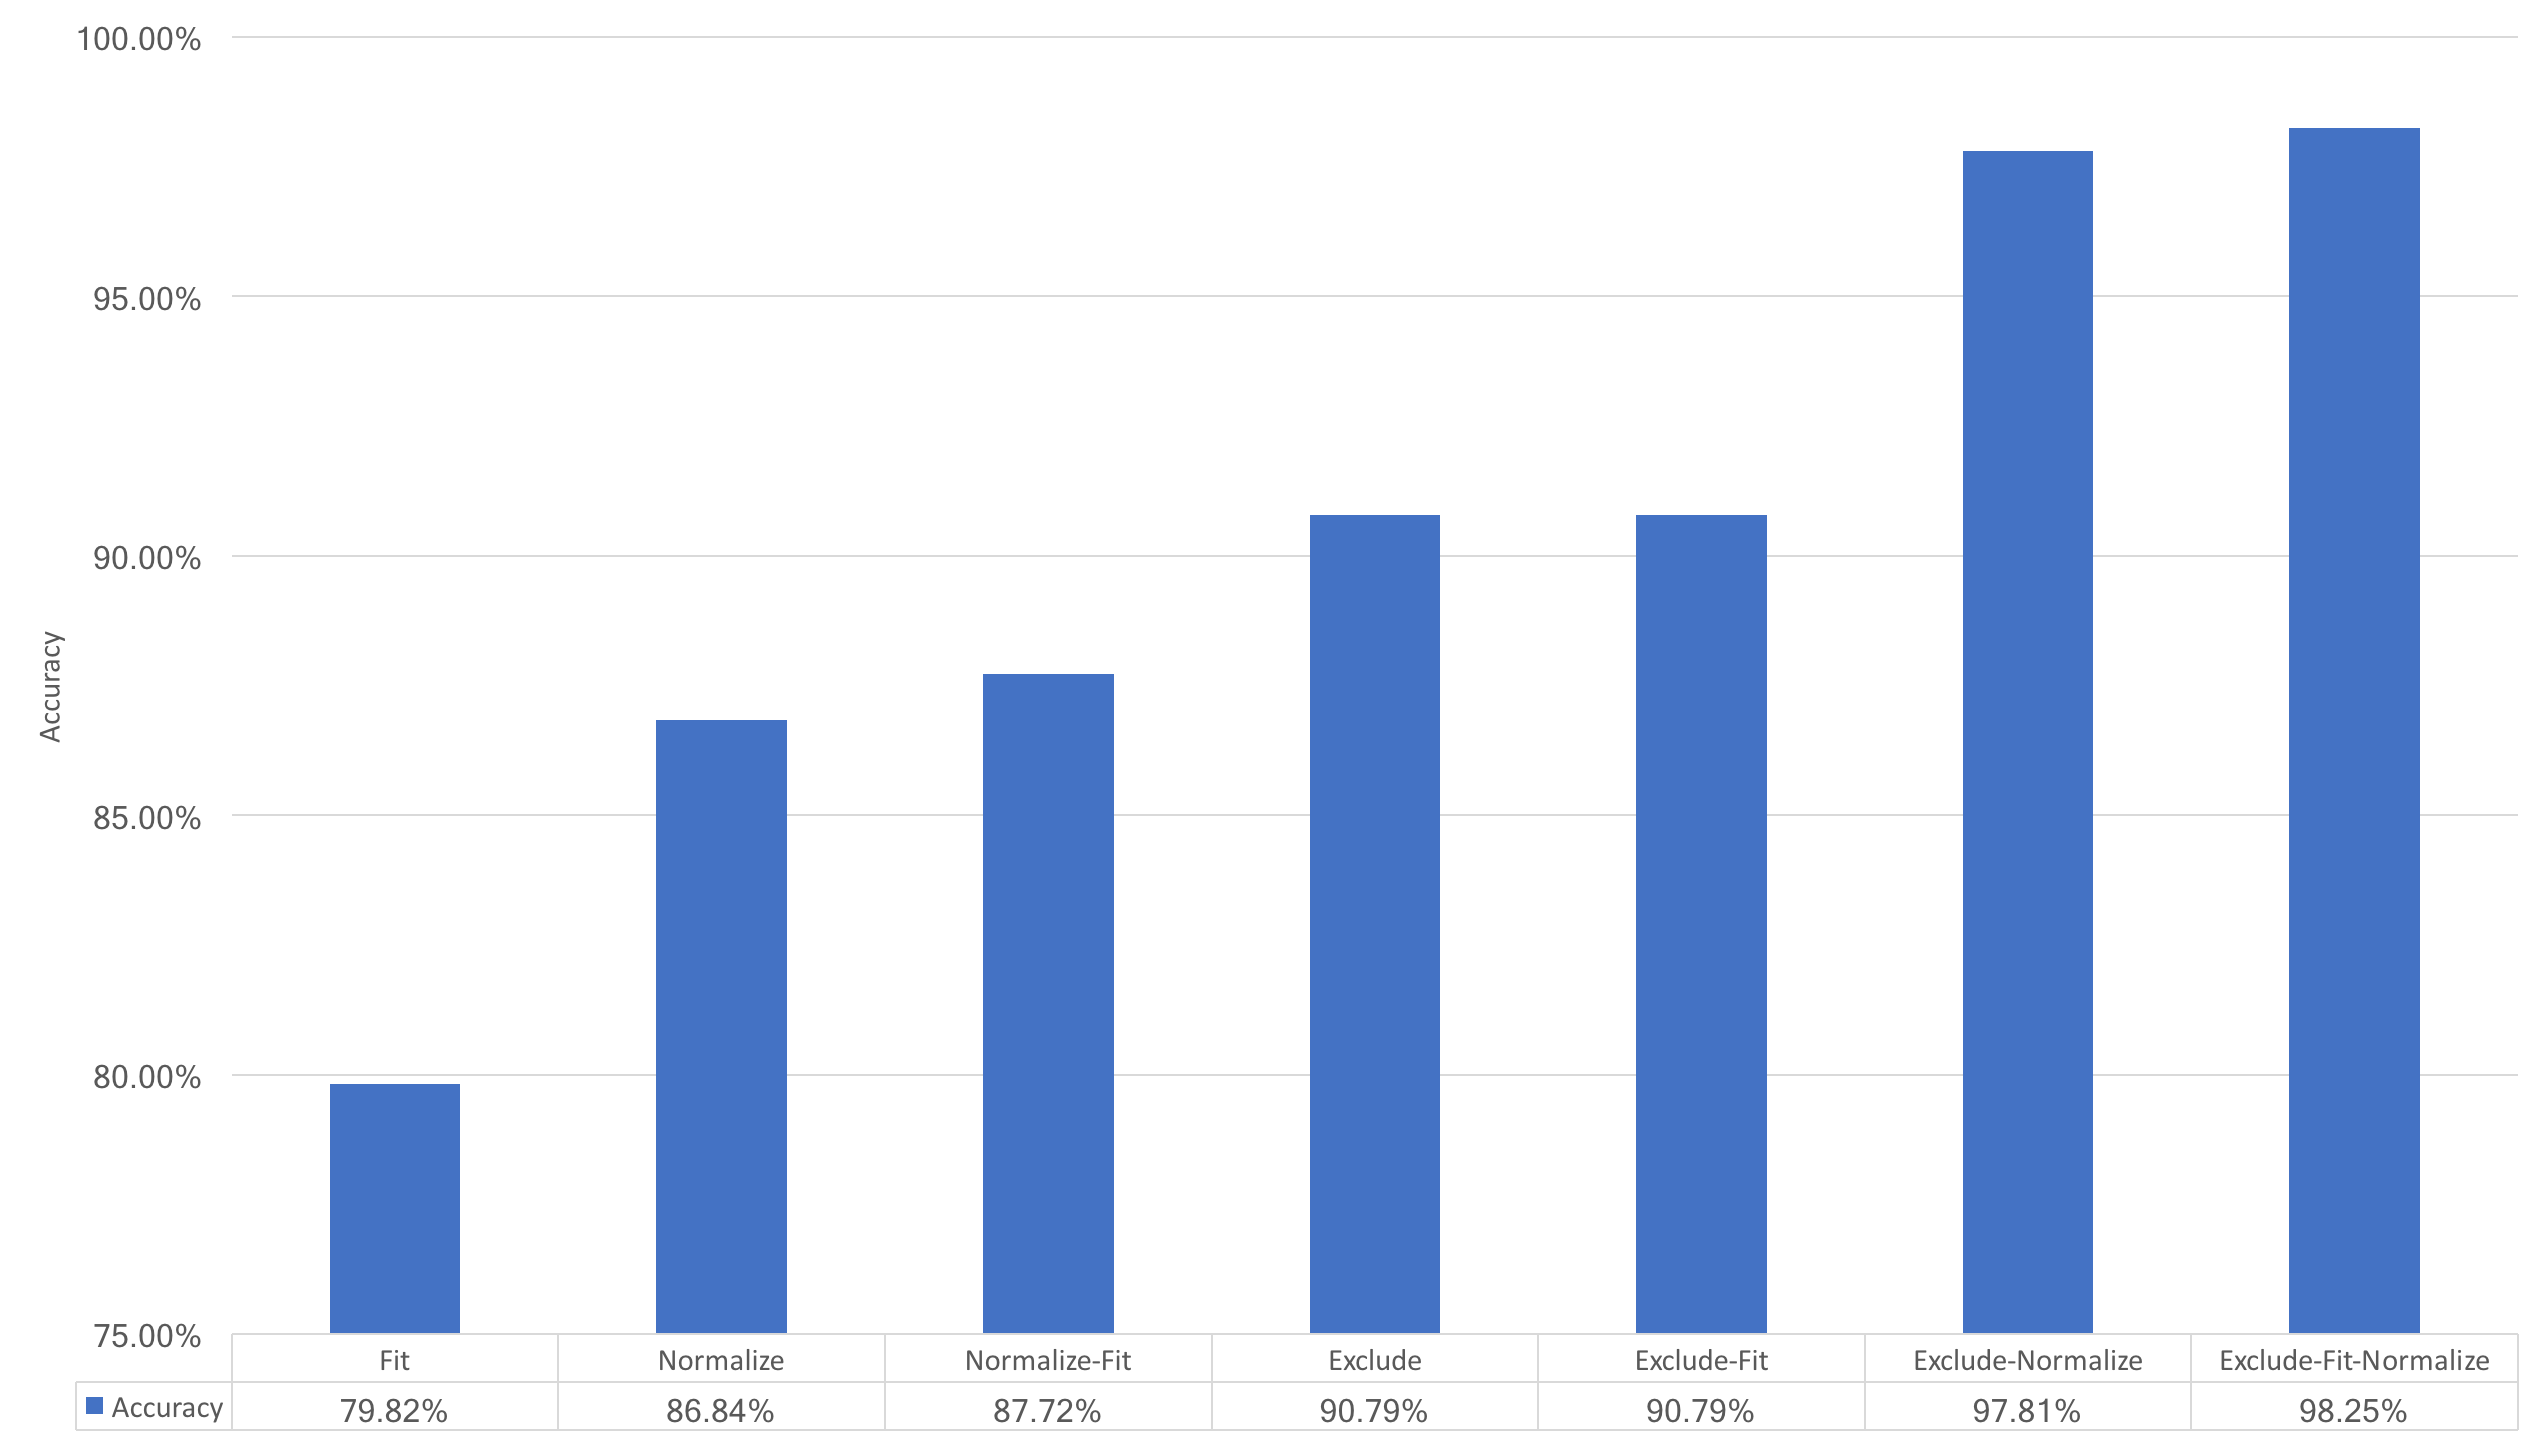
\includegraphics[width=\linewidth ]{figure/acc-data}}
\caption{Accuracy Comparison over Different Data Process Methods}
\label{fig_f0fit}
\end{figure}

\begin{figure}[H]
\begin{minipage}{0.5\linewidth}
\centerline{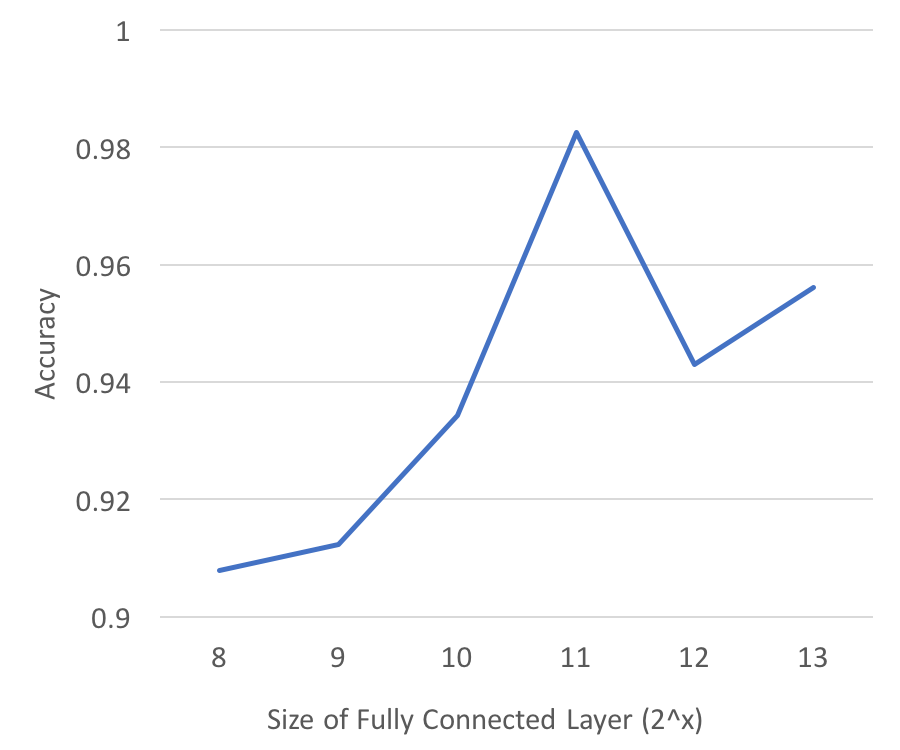
\includegraphics[width=\linewidth ]{figure/acc-width}}
\end{minipage}
\hfill
\begin{minipage}{0.5\linewidth}
\centerline{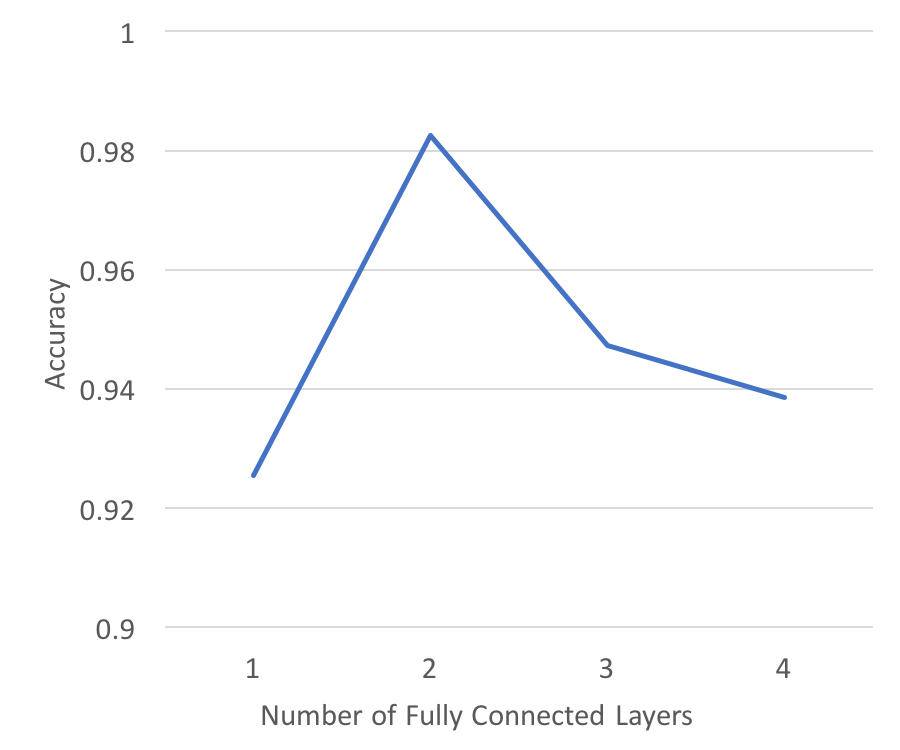
\includegraphics[width=6.0cm]{figure/acc-depth}}
\end{minipage}
\caption{Accuracy Comparison over Different Network Widths(Left);
Accuracy Accuracy Comparison over Different Network Depths(Right)}
\label{fig_f0fit}
\end{figure}

\begin{figure}[H]
\begin{minipage}{0.6\linewidth}
\centerline{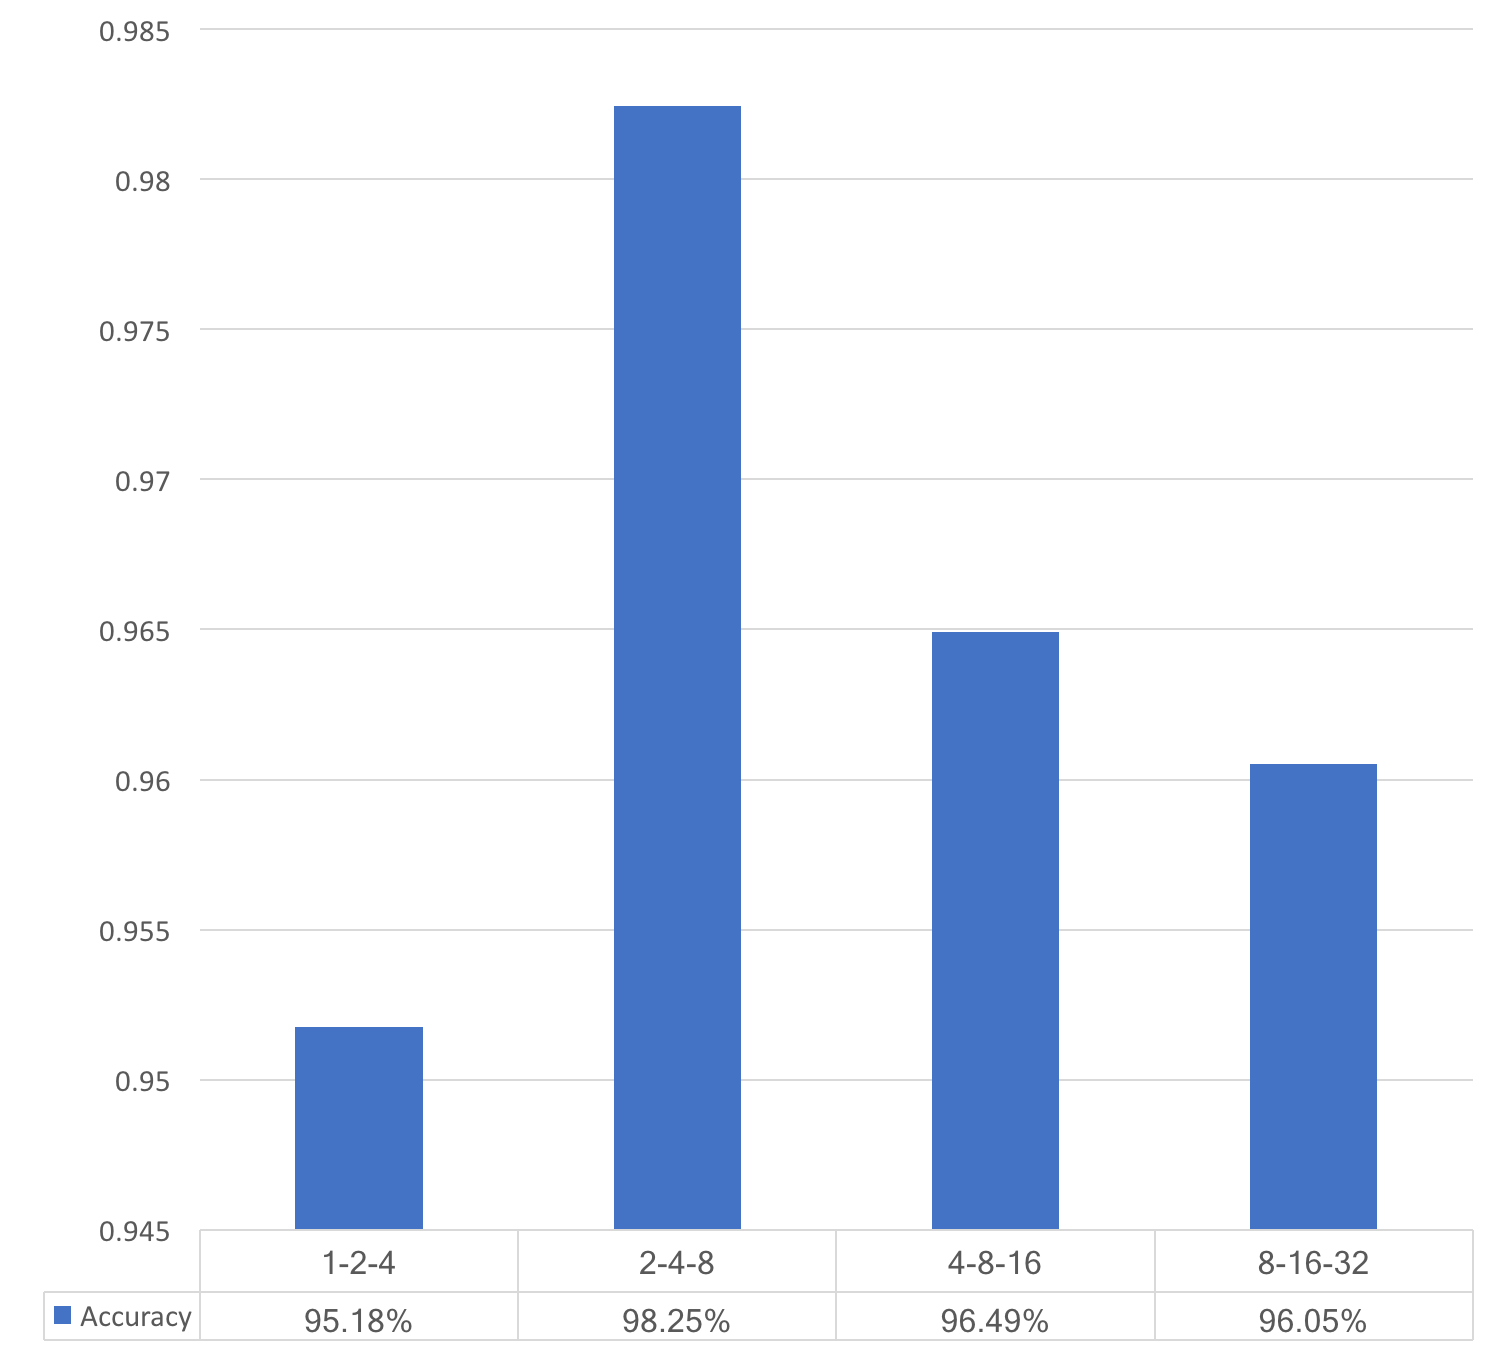
\includegraphics[width=6.0cm ]{figure/acc-channel}}
\end{minipage}
\hfill
\begin{minipage}{0.5\linewidth}
\centerline{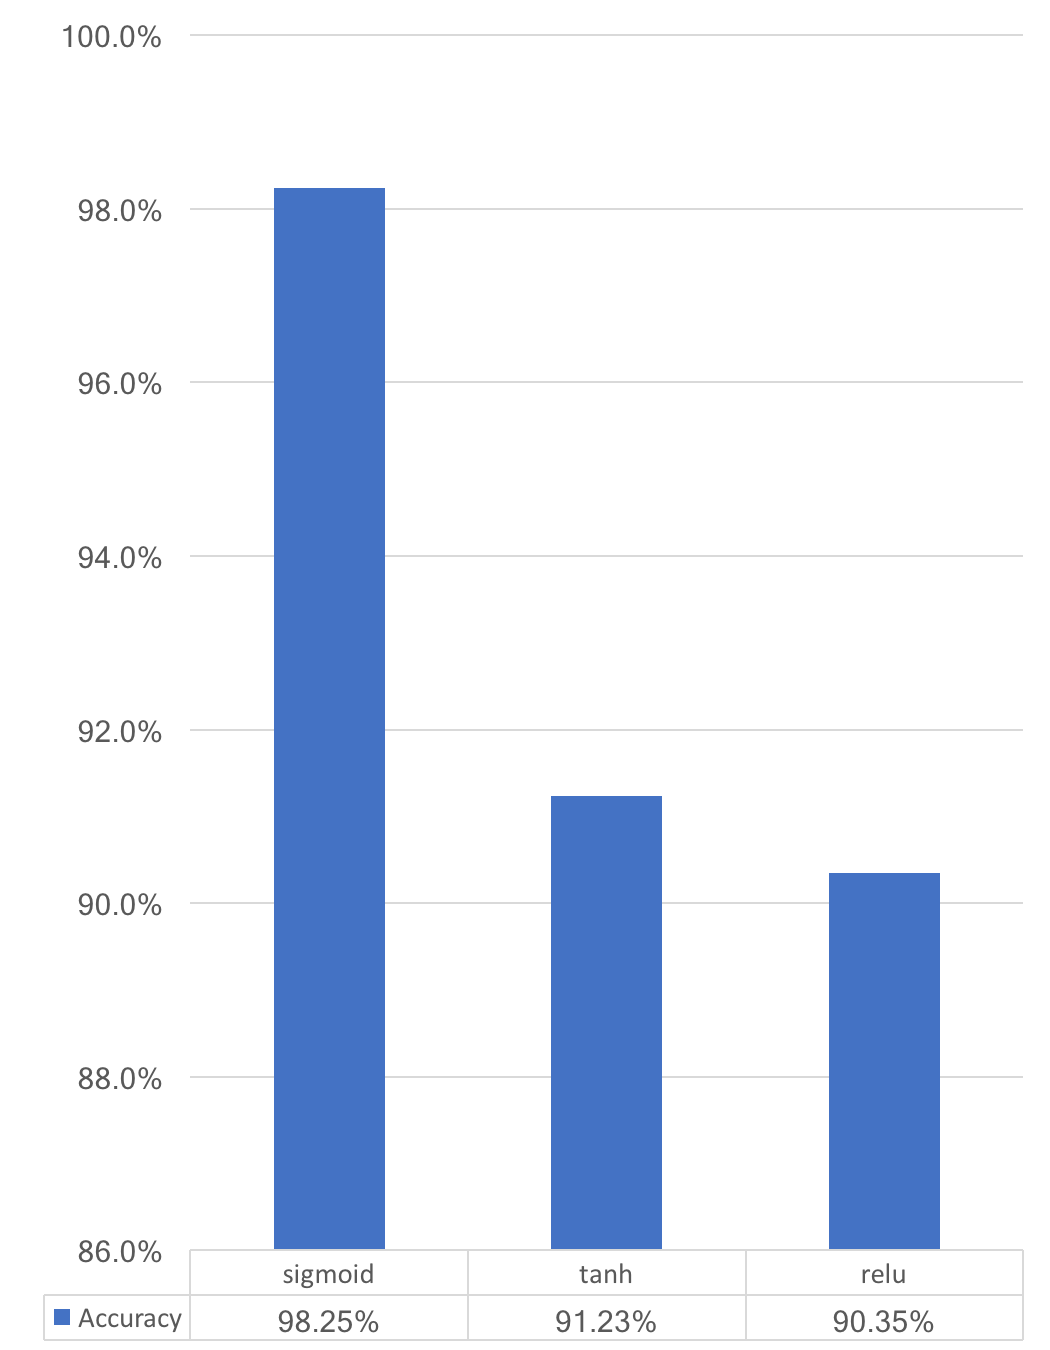
\includegraphics[width=4.25cm]{figure/acc-activation}}
\end{minipage}
\caption{Accuracy Comparison over Different Number of Filters(Left); 
Accuracy Comparison over Different Activation Functions(Right);}
\label{fig_f0fit}
\end{figure}


\subsection{Compare over Different Deep Learning Toolkits}
In our experiments, we compared the efficiency, accuracy and stability on GPU computation of three mainstream deep learning toolkits: CNTK\cite{dallycntk} , mxnet\cite{chen2015mxnet} and torch\cite{collobert2011torch7} . 
\begin{enumerate}
	\item \textit{Efficiency}: In our experiments, we implemented our model in three toolkits and evaluated the training time of 60 epochs with mini-bash size of 10. Figure 8 shows the comparison of training time over three toolkits. Table 1 shows the comparison of GPU utilization over three toolkits. From the figure we find that torch and mxnet are significantly more efficient than CNTK, and torch is a little better than mxnet. Possible reasons include:
	\begin{enumerate}
		\item Torch has a significantly better ability to make full use of GPU.
		\item mxnet has better algorithms so can reach a better efficiency with less GPU resources.
	\end{enumerate}
	\item \textit{Accuracy}: We evaluate the same model implemented in three toolkits and compared their accuracy. Figure 8 shows the comparison of accuracy over three toolkits and the relationship between accuracy and efficiency. From the figure we find that CNTK has a better performance than mxnet and torch. We discover that the frame work with higher efficiency tends to have a lower accuracy, the possible reason is that the different toolkits have different balances of efficiency and accuracy.
	\item \textit{Stability}: During our experiments, we find that CNTK and mxnet has better numerical stability than torch. For the same toolkit, the numerical stability on CPU is better than that on GPU.
\end{enumerate}

\begin{figure}[H]
\centerline{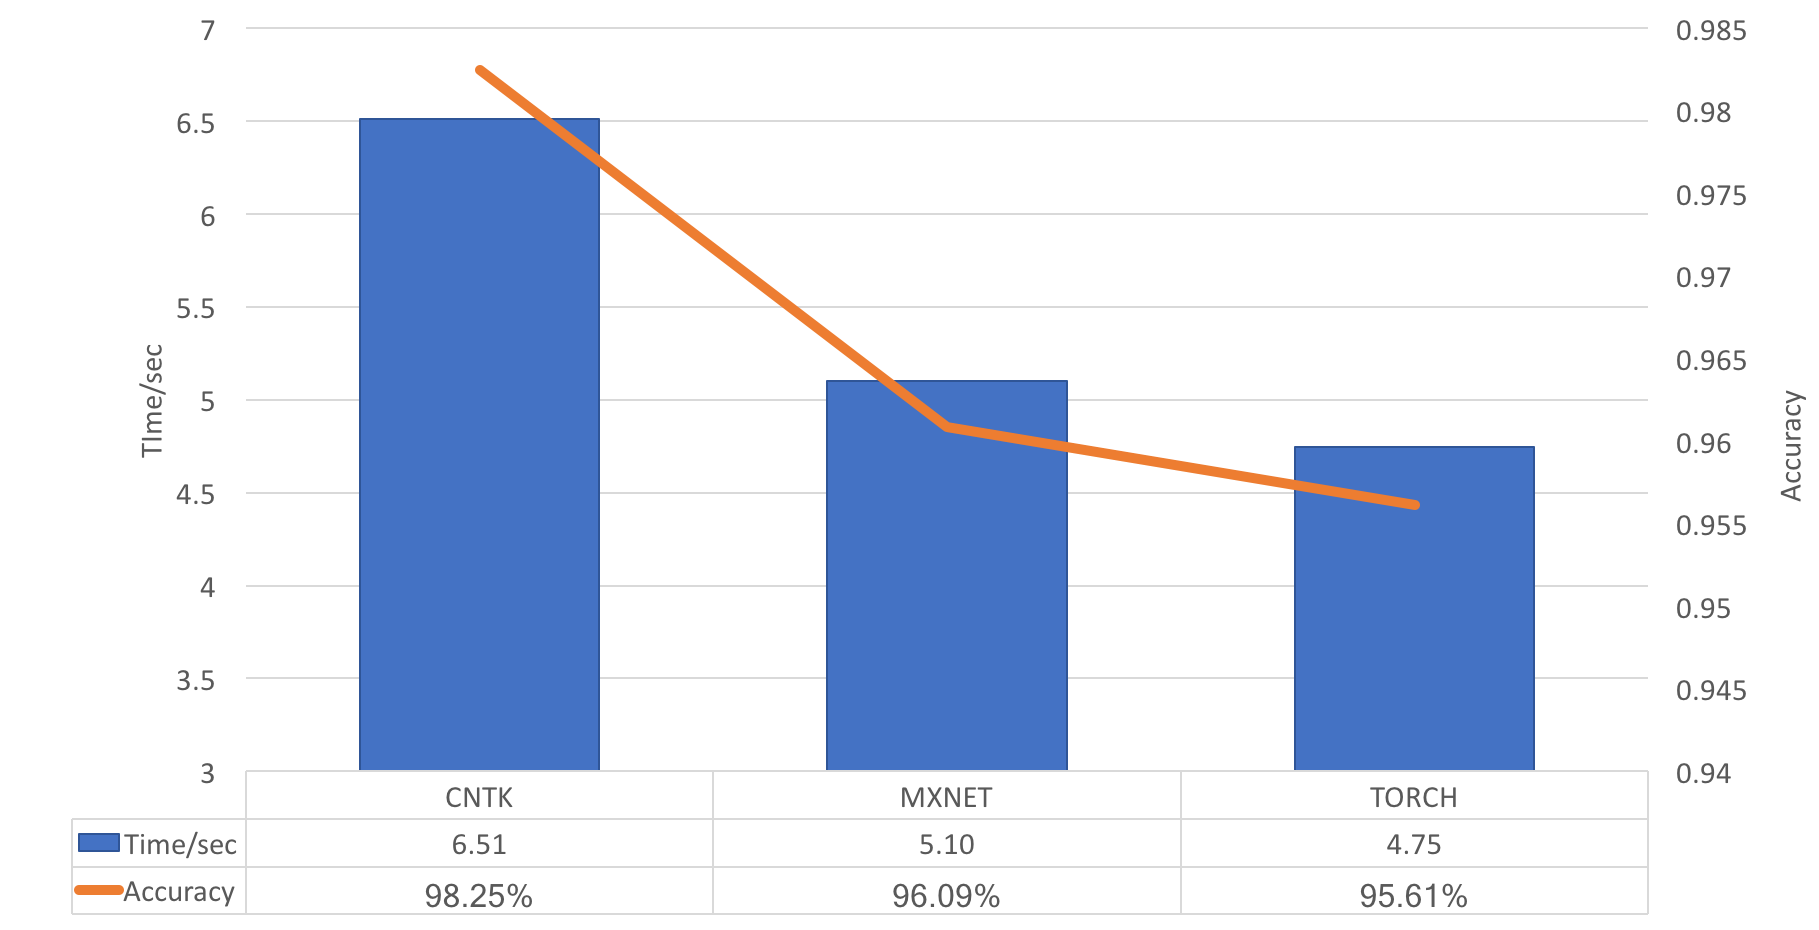
\includegraphics[width=\linewidth ]{figure/acc-time}}
\caption{Comparison of Training Time and Accuracy over Different Toolkits}
\label{fig_f0fit}
\end{figure}

\begin{table}[H]
\centering
\begin{tabular}{l|l|l|l}
         & CNTK       & mxnet      & torch      \\ \hline
GPU-Util & $\sim$67\% & $\sim$57\% & $\sim$80\%
\end{tabular}
\caption{GPU Utilization Comparison over Different Toolkits}
\label{my-label}
\end{table}

\newpage

\section{Conclusion}
In this work, we proposed a CNN-based model for Chinese Mandarin tone classification and a series of methods to process input data. 
We chose the classification accuracy as our main evaluation metric and explored the impacts of different data processing methods, network architectures and deep learning toolkits. Furthermore, we explored the performances of three mainstream deep learning toolkits: CNTK, mxnet and torch in the aspect of efficiency, accuracy, stability and availability.


\bibliographystyle{plain}
\bibliography{rep}

\end{document}